\chapter{評価}
本章では,全章で提案したヘッドノードにおけるフレーム処理並列化の有効性を確認するため,ヘッドノード内に構築したコンテナ環境において2種類の実験 (実験1, 実験2)を行う.
実験1では,提案手法は既存手法と比較してヘッドノード内でのフレーム処理時間が短縮されているかを確認する.実験2では,ヘッドノードの各CPUコアの使用率を計測し,提案手法を用いてもうちくしたマルチディスプレイシステムのスケーラビリティについての確認を行う.
本章では,まず4.1節で,分評価で利用した実験環境について説明する.次に,4.2節で,実験1における実験方法と実験結果について述べる.さらに,4.3節では,実験2における実験方法と実験結果を述べる.

\section{実験環境}
本実験で用いたヘッドノード内のコンテナ構成を図4.2に示す.
当実験環境は,ヘッドノードとして用いるデスクトップPC内のコンテナ仮想環境を用いて構築したものである.
実験環境内では1つの分割コンテナと複数の圧縮コンテナを用意する.
また,本実験では様々な画面構成のマルチディスプレイを構築することを想定し,圧縮コンテナの数は構成ディスプレイと同じ数になるように増減させる.
本実験では1面,2面,4面,6面,9面構成のそれぞれのマルチディスプレイを構築することを想定し,評価を行った.

\begin{table}[H]
    \caption{ヘッドノード用デスクトップPCの仕様}
    \begin{center}
    \begin{tabular}{cc}
    \hline
    要素 & 仕様 \\\hline\hline
    CPU & i7-5960X (3.0 GHz×8) \\ \hline
    メモリ & 64.0 GB \\ \hline
    通信帯域 & 1 Gbps \\ \hline
    OS & CentOS 7.3 \\ \hline

    \end{tabular}
    \end{center}
\end{table}

評価に用いる映像としては,クリエイティブ・コモンズ・ライセンスのもとで利用できる3DアニメーションであるBig Buck Bunny \cite{bigbackbunny}を使用した.
表4.4に,Big Buck Bunnyのプロパティを示す.
さらに,図4.3にBig Buck Bunny再生時のスクリーンショットを示す.

\begin{table}[htbp]
    \caption{Big Buck Bunnyのプロパティ}
    \begin{center}
    \begin{tabular}{cc}
    \hline
    項目 & 内容 \\\hline\hline
    動画形式 & MP4 \\ \hline
    コーデック & H.264 \cite{h264} \\ \hline
    長さ & 10分34秒 \\ \hline
    総フレーム数 & 19020枚 \\ \hline
    フレームレート & 30 fps \\ \hline
    解像度 & 4K (3840×2160) \\ \hline

    \end{tabular}
    \end{center}
\end{table}

\begin{figure}[H]
    \hspace*{\fill}
    \includegraphics[width=\linewidth]{./fig/chap4/bigbuckbunny.eps}
    \hspace*{\fill}
    \caption{Big Buck Bunnyのスクリーンショット}
   \end{figure}

ヘッドノードで行われる処理の実装には,OpenCV \cite{opencv}, libjpeg-turbo ~\cite{libjpeg}, Boost.Asio \cite{asio}という3種類のライブラリを利用した. 
OpenCVは画像処理ライブラリ,libjpeg-turboはJPEGの圧縮と展開を行うライブラリ,Boost.Asioはソケット通信を行うライブラリである.
また,ディスプレイノードの処理の実装にはlibjpeg-turbo, Boost.Asio, fbdevを利用した.
実装にはC++言語を使用し,GCCコンパイラ (GNU C Compiler) \cite{gcc}でコンパイルを行った.

\begin{figure}[H]
    \hspace*{\fill}
    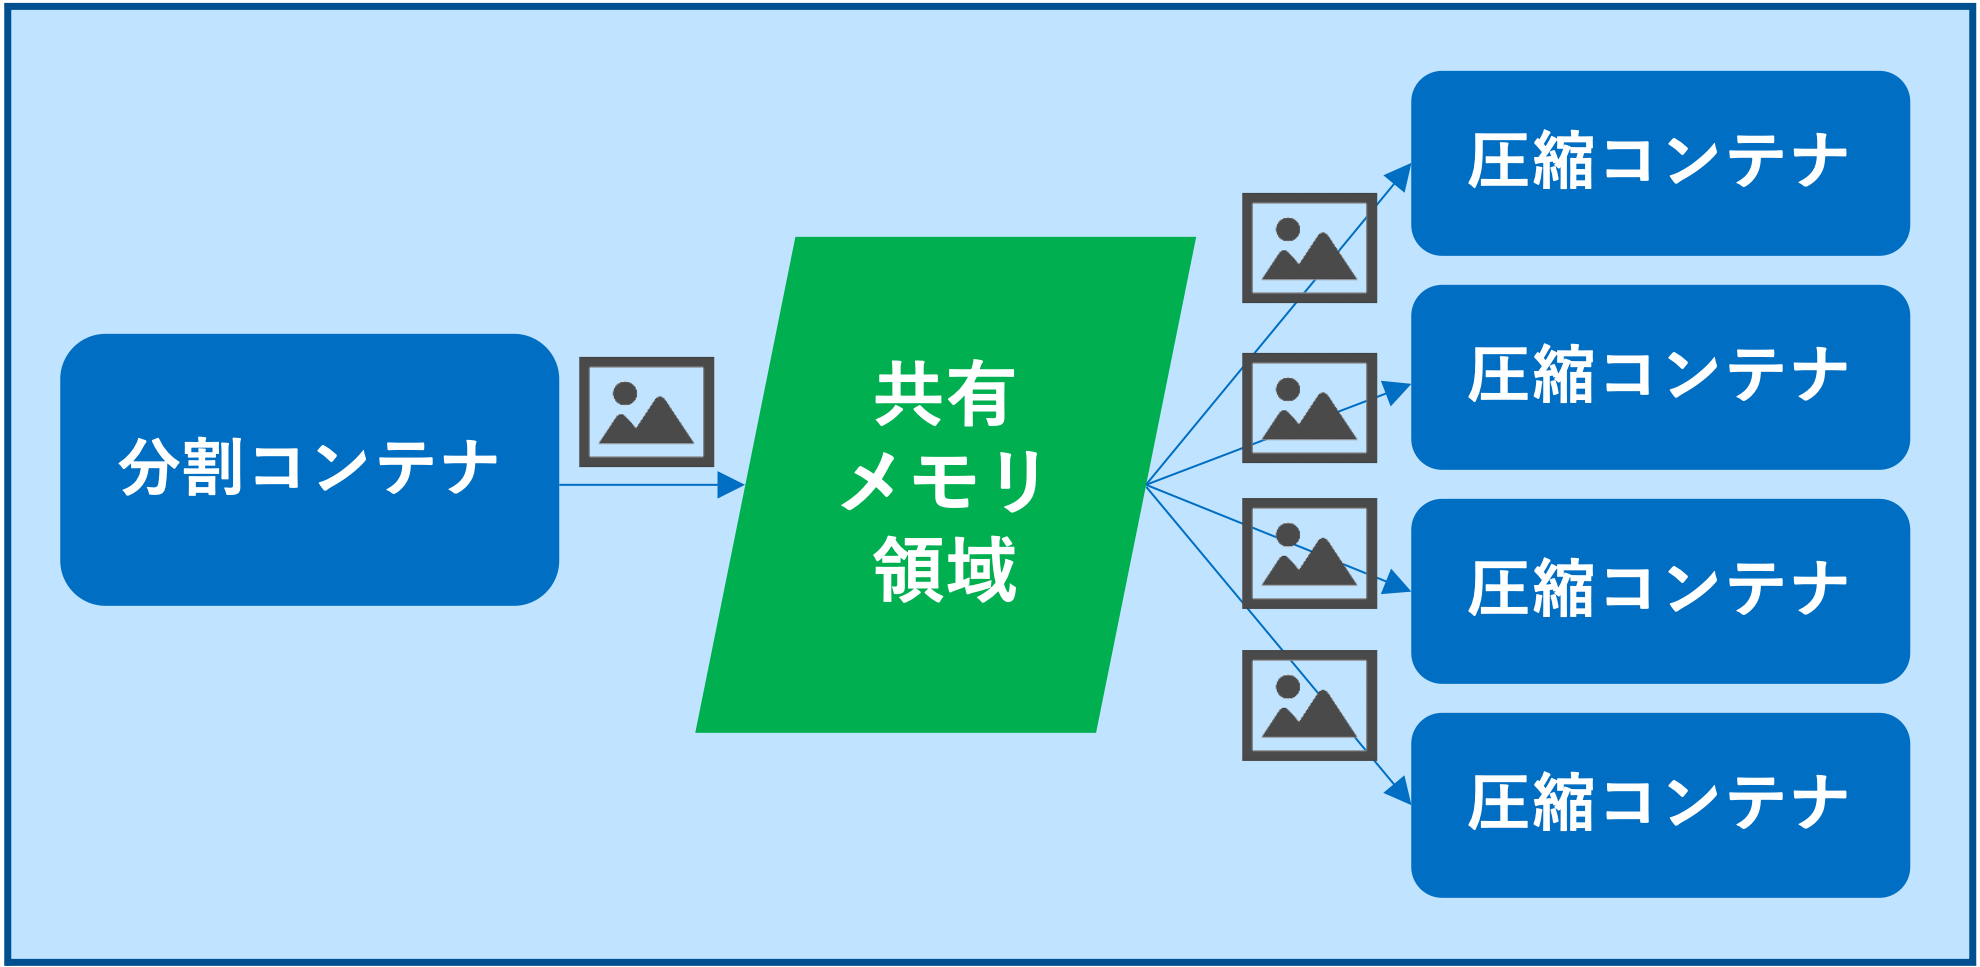
\includegraphics[width=\linewidth]{./fig/chap4/evaluation_environment.eps}
    \hspace*{\fill}
    \caption{実験環境のコンテナ構成}
   \end{figure}

\section{フレーム処理時間の評価}

\subsection{実験方法}
先行研究で提案された手法と提案手法において,4面構成のMDを想定した環境で4K解像度の画像を表示し,動画のフレーム開始から1000フレーム目の処理が終了するまでの1フレームあたりに要するフレーム処理時間を計測した.
また,フレーム処理時間の計測にはC++11の時間ライブラリであるchronoを用いた.
図4.6に先行研究で提案されたシステムと提案手法でのフレーム処理時間を示す.

\subsection{実験結果}

既存手法ではヘッドノードでのフレーム処理時間の平均が52.35msであったのに対し,提案手法では21.72msとなっており,フレーム処理時間が既存手法と比較して40\%程度まで短縮された事が確認できた.

また,本提案で新たに生じた処理である共有メモリを用いたプロセス間での画像フレームデータ受け渡しに要する時間も平均で1ms未満となっており,オーバーヘッドは非常に小さくなっていることも確認できる.

以上の結果より,フレーム処理プロセスの並列化を行った提案手法によって,システムのボトルネックが解消された.

\begin{figure}[H]
    \hspace*{\fill}
    \includegraphics[width=\linewidth]{./fig/chap4/processing_time_4.eps}
    \hspace*{\fill}
    \caption{フレーム処理時間の比較 (4面構成時)}
\end{figure}

\begin{figure}[H]
    \hspace*{\fill}
    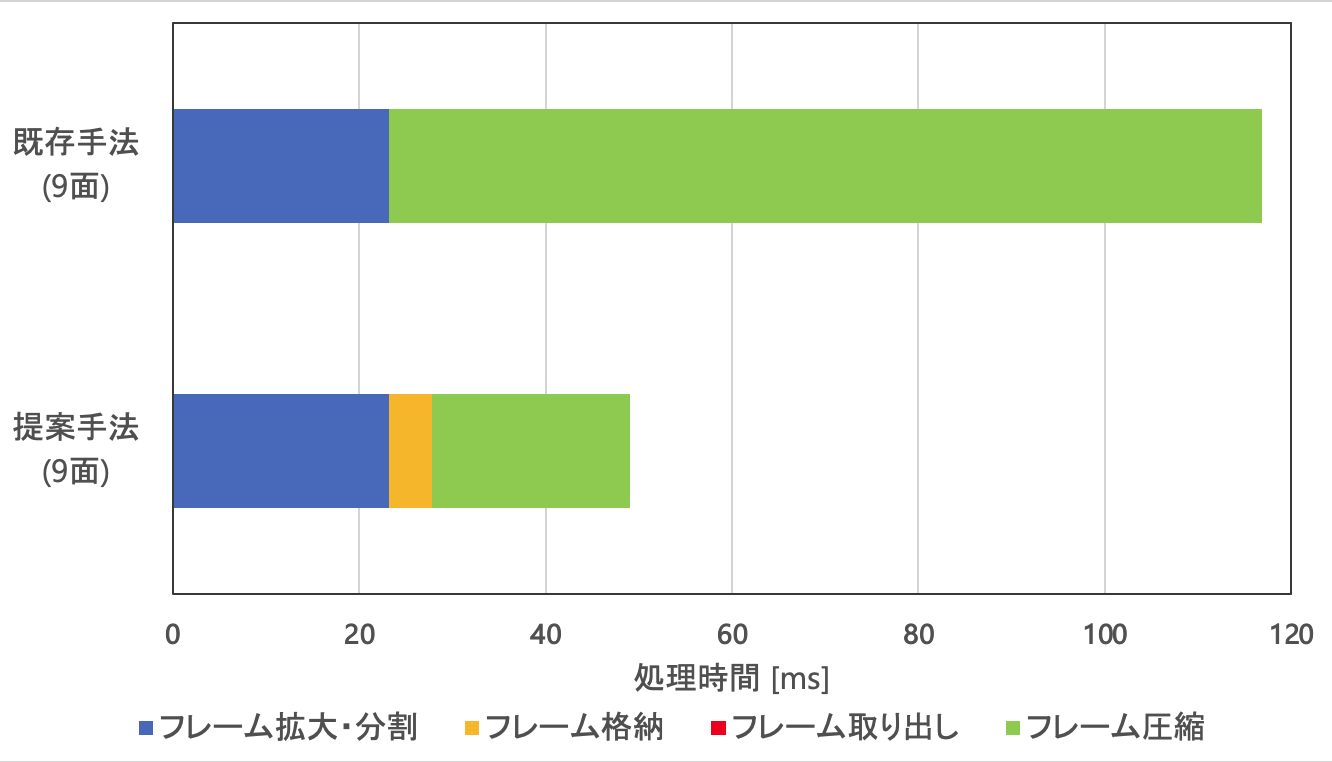
\includegraphics[width=\linewidth]{./fig/chap4/processing_time_9.eps}
    \hspace*{\fill}
    \caption{フレーム処理時間の比較 (9面構成時)}
\end{figure}

\section{フレーム処理速度の評価}



\subsection{実験方法}

\subsection{実験結果}

\subsection{結果に対する考察}